%\documentclass[eng,final, oneside, printmode]{mgr} %mwbk
\documentclass[pl,final,oneside]{mgr} %printmode
\usepackage[polish]{babel}
\usepackage{polski}
\usepackage[OT4]{fontenc}
\usepackage[utf8]{inputenc}
\frenchspacing

\usepackage{cmap}
\linespread{1.1} %interlinia
\usepackage{amsmath}
\usepackage{amsfonts}
\usepackage{latexsym}
\usepackage{longtable}
\usepackage{graphicx} 
\usepackage{geometry}
\usepackage{pgfplots}
\usepackage{multirow}
\setlength{\parindent}{0pt}
\setlength{\parskip}{1ex plus 0.5ex minus 0.2ex}
\pgfplotsset{compat=1.13}
\usepackage{bookmark}
\usepackage{listings}
\usepackage{indentfirst}
\setcounter{secnumdepth}{6}
\usepackage{textcomp}
\usepackage[nottoc,numbib]{tocbibind}

\setlength{\parindent}{30pt}

\setlength{\parskip}{0pt}

\bookmarksetup{
	open,
	addtohook={%
		\ifnum\bookmarkget{level}<1 %
		\bookmarksetup{bold}%
		\fi
	},
}

\hypersetup{%
	colorlinks = true,
	linkcolor  = black
}

%\newgeometry{tmargin=1.5cm, bmargin=1.5cm, lmargin=1.5cm, rmargin=1.5cm}

% Default fixed font does not support bold face
\DeclareFixedFont{\ttb}{T1}{txtt}{bx}{n}{9} % for bold
\DeclareFixedFont{\ttm}{T1}{txtt}{m}{n}{9}  % for normal

% Custom colors
\usepackage{color}
\definecolor{deepblue}{rgb}{0,0,0.5}
\definecolor{deepred}{rgb}{0.6,0,0}
\definecolor{deepgreen}{rgb}{0,0.5,0}

\usepackage{listings}
\lstset{language=Bash,
	basicstyle=\scriptsize\ttfamily,
	rulecolor=\color{black},
	upquote=true,
	numbersep=8pt,
	showstringspaces=false,
	breaklines=true,
	frameround=ftff,
	frame=single,
	belowcaptionskip=5em,
	aboveskip=1em,
	belowskip=1em,
}


%\renewcommand\lstlistingname{Dodatek A - spis listingów}
%\renewcommand\lstlistlistingname{{Dodatek A - spis listingów}}

\author{Rafał Dziwiński}
\title{Analiza możliwości i implementacja niezawodnego routingu w wirtualnym środowisku High Avability przy wykorzystaniu platformy Kubernetes oraz Calico.}

\engtitle{Analysis of possibilities and implementation of reliable routing in the virtual High Avability environment using the Kubernetes and Calico platforms.}
\supervisor{dr inż. Waldemar Grzebyk, KTT}
\field{Telekomunikacja}
\specialisation{Teleinformatyka i multimedia}

% \renewcommand*\thesection{\arabic{section}.} % zmiana numeracji sekcji 0.X -> X
\begin{document}

\maketitle
\tableofcontents

\chapter{Wstęp}
Jeszcze kilka lat temu chcąc wdrożyć zaawansowaną aplikację rozdzielając poszczególne procesy używano maszyn wirtualnych. Był to najlepszy sposób na izolację procesów mogących w niepożądany sposób wpływać na siebie nawzajem. Takie rozwiązanie umożliwiało przeniesienie usługi do chmury. Pozwalało to na delegowanie odpowiedzialności za infrastrukturę fizyczną firmie trzeciej. Obecnie nowoczesne aplikacje tworzone są jako szereg współpracujących ze sobą mikroserwisów i umieszczane w kontenerach. Coraz więcej firm decyduje się na uruchomienie swoich aplikacji w chmurze, poza swoją infrastrukturą co przynosi wiele niekwestionowanych korzyści. Dynamiczny rozwój tej dziedziny przyczynił się do stworzenia takich rozwiązań jak Docker oraz Kubernetes.

Zmiany na rynku zachodzą również w branży sieciowej. Coraz więcej mówi się o Software Definied Network oraz o końcu konfiguracji urządzeń przez CLI. Wielu producentów tworzy API (Interfejs programowania aplikacji) do swoich urządzeń oraz zachęca do ich konfiguracji w ten sposób. Jednym z wielu rozwiązań zapewniających routing w środowiskach zwirtualizowanych jest Calico.  Możliwe jest połączenie dwóch obecnie najpopularniejszych trendów w branży IT? Celem pracy jest odpowiedź na to pytanie. Ponadto zostanie poddane analizie możliwość stworzenia rozwiązania niezawodnego routingu w środowisku zwirtualizowanym. Jako orkiestrator kontenerów wykorzystano platformę Kubernetes. Sieć zostanie zbudowana przy wykorzystaniu narzędzi Calico oraz BIrd.

\chapter{Cel i zakres pracy}

%Aspekt badawczy:
%1. Opracowanie zakresu analizy oraz kryteriów oceny.
%2. Analiza możliwości implementacji niezawodnego routingu w wirtualnym środowisku High Avability przy
%wykorzystaniu platformy Kubernetes oraz Calico:
%a) analiza sposobów implementacji niezawodnego routingu w środowisku wirtualnym,
%b) porównanie rozwiązania zwirtualizowanego do fizycznego w oparciu o przyjęte kryteria.
%Aspekt inżynierski:
%1. Przygotowanie środowiska testowego wykorzystującego platformę Kubernetes oraz implementacja wirtualnych
%routerów jako kontenerów przy pomocy aplikacji Docker.
%2. Przygotowanie scenariuszy i procedur testowych.
%3. Przeprowadzenie testów dotyczących czasu odzyskania pełnej funkcjonalności sieci w momencie awarii jednego
%bądź wielu z jej elementów.
%Zadania do wykonania:
%1. Studia literaturowe.
%2. Opracowanie zakresu analizy oraz kryteriów oceny.
%3. Analiza możliwości implementacji niezawodnego routingu w wirtualnym środowisku High Avability przy
%wykorzystaniu platformy Kubernetes oraz Calico:
%a) analiza sposobów implementacji niezawodnego routingu w środowisku wirtualnym,
%b) porównanie rozwiązania zwirtualizowanego do fizycznego w oparciu o przyjęte kryteria.
%4. Przygotowanie środowiska testowego wykorzystującego platformę Kubernetes oraz implementacja wirtualnych
%routerów jako kontenerów przy pomocy aplikacji Docker.
%5. Przygotowanie scenariuszy i procedur testowych.
%6. Przeprowadzenie testów dotyczących czasu odzyskania pełnej funkcjonalności sieci w momencie awarii jednego
%bądź wielu z jej elementów.
%7. Opracowanie wniosków z przeprowadzonej analizy i testów.
\chapter{Część teoretyczna}
\section{Słownik pojęć}
\begin{description}
\item[Pod] najmniejsza możliwa do wdrożenia jednostka obliczeniowa, zarządzana przez platformę Kubernetes.
\item[Node] maszyna robocza zawierająca usługi niezbędne do uruchamiania podów oraz zarządzania nimi.
\item[Master nod] maszyna robocza, zapewniająca płaszczyznę sterowania klastra.
\item[Worker node] maszyna robocza, zapewniająca zasoby sprzętowe dla tworzonych podów.
\item[Host endpoint] reprezentuje jeden bądź wiele fizycznych, wirtualnych interfejsów połączonych z hostem, na którym uruchomione jest calico.
\item[Workload endpoints] reprezentuje zasób wirtualny, podłączony do sieci Calico.
\item[Control plane] płaszczyzna sterowania zapewniająca logikę działania systemu.
\end{description}
\section{Konteneryzacja}
Aby opisać w dobry sposób konteneryzację, warto przypomnieć sobie jak było kiedyś. Pierwszą metodą wdrażania aplikacji, było uruchomienie każdej z nich na osobnym fizycznym serwerze. Niestety, w tym przypadku nie ma możliwości wydzielenia zasobów dla danej aplikacji. Powoduje to problemy z jednoczesnym uruchomieniem wielu aplikacji. Może się zdarzyć tak, że duże obciążenie na przykład przez atak DDoS spowoduje zatrzymanie pracy innych, zupełnie niezwiązanych ze sobą usług. Jedynym wyjściem jest uruchomienie aplikacji na osobnych fizycznych maszynach, jednak generuje to szereg problemów. Między innymi:
\begin{itemize}
	\item Trudność w skalowaniu zasobów;
	\item zwiększenie ilości niewykorzystanych zasobów;
	\item duże koszty.
\end{itemize}
Wprowadzono pojęcie wirtualizacji, aby temu zaradzić. Pozwala ona na uruchomienie wielu wirtualnych maszyn (VM), na jednym fizycznym serwerze. Dzięki temu możliwa jest separacja aplikacji co ma wpływ na stabilność w przypadku przeciążenia jednej z aplikacji oraz bezpieczeństwo. Kolejnym plusem jest możliwość lepszego zarządzania oraz skalowania zasobów sprzętowych. Zmniejsza również koszt wdrożenia oraz utrzymania dzięki możliwości zastosowania jednego, wydajnego serwera oraz ograniczenie kosztu prądu. W tym przypadku każda z VM wirtualizuje fizyczne zasoby oraz sprzęt co również nie jest rozwiązaniem w stu procentach wydajnym.

Na pomoc przychodzi tak zwana konteneryzacja. Jest to rozwiązanie podobne do maszyn wirtualnych, z tą różnica, że nie jest potrzebna wirtualizacja sprzętu oraz systemu operacyjnego. Kontener działa na jądrze systemu hosta oraz jego zasobach które nie są wirtualizowane. Oznacza to, że w przypadku wdrożenia aplikacji, w kontenerze potrzebne jest jedynie dodanie do niego pakietów przez nią wymaganych. Na przykład, w momencie uruchomienia dystrybucji Fedora na fizycznym serwerze z Debianem kontener będzie zawierał jedynie pakiety charakterystyczne dla tej pierwszej. W ogromnych skrócie można powiedzieć, że jest to lżejsza wersja VM. Ponadto użycie ich użycie niesie za sobą wiele zalet:
\begin{itemize}
	\item Większa łatwość i wydajność tworzenia obrazu kontenera w porównaniu do użycia obrazu VM.
	\item Łatwiejszy rozwój aplikacji przez możliwość szybkiego budowania kolejnych obrazów.
	\item Możliwość łatwiej migracji między wieloma różnymi usługami w chmurze.
	\item Centralne monitorowanie oraz administracja kontenerami.
	\item Wydajniejsze oraz efektywniejsze zarządzanie zasobami sprzętowymi.
	
\end{itemize}
Różnicę między tradycyjnym wdrażaniem aplikacji, a VM oraz kontenerami, najlepiej obrazuje i podsumowuje poniższa grafika: 
\begin{figure}[h!]
	\centering
	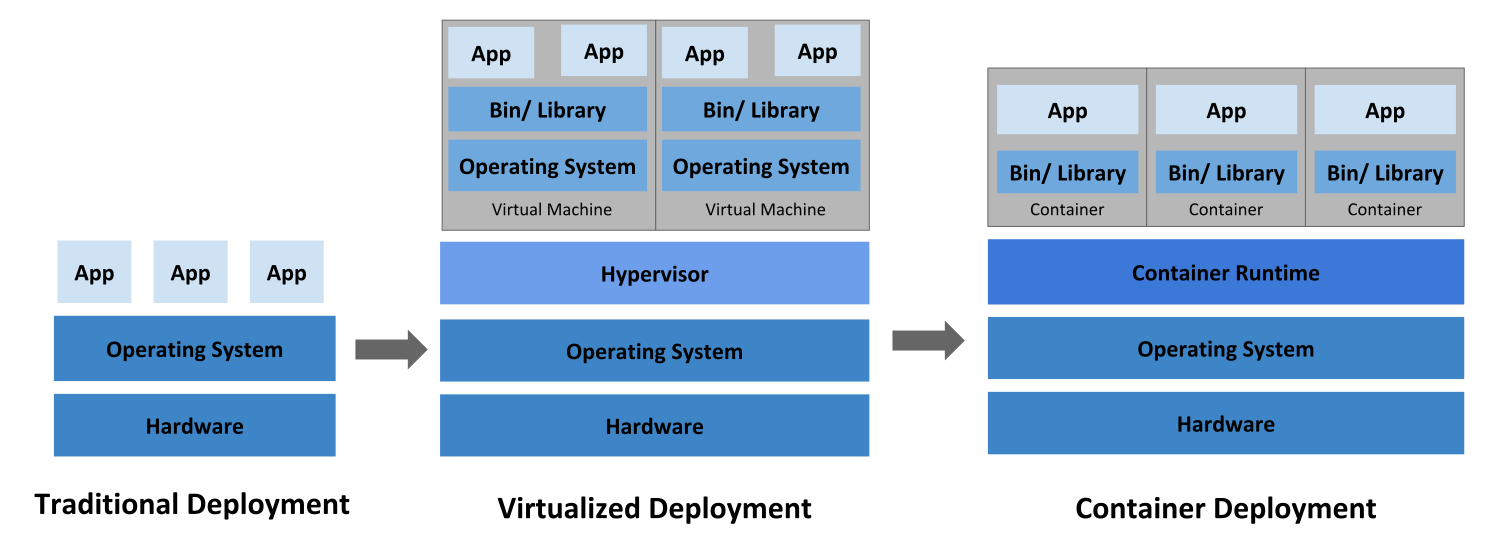
\includegraphics[width=1\linewidth]{images/container_evolution}
	\caption{Ewolucja możliwości wdrażania aplikacji \cite{kube_doku}.}
	\label{fig:container_evolution}
\end{figure}
\section{Kubernetes}
Słowo Kubernetes wywodzi się z języka greckiego i oznacza sternika, bądź pilota. Pierwsze linie kodu, napisane przez Google Inc. pojawiły się już w 2004 roku. Platforma bazuje na wieloletnim doświadczeniu tej firmy oraz społeczności.

Jest to otwarta platforma, służąca do zarządzania skonteneryzowanymi aplikacjami oraz usługami. Głównym jej celem jest ułatwienie i automatyzacja ich wdrożeń bądź konfiguracji. Obecnie społeczność, a także firmy stojące za rozwojem systemu są na tyle liczne, że z powodzeniem ta młoda platforma może być wdrażana w środowiskach produkcyjnych.

Jak wspomniano w poprzednim rozdziale, najlepszym z rozwiązań do uruchamiania aplikacji są kontenery. W środowisku produkcyjnym, liczącym ich wiele dziesiątek bądź też setek, ręczne zarządzanie nimi jest niewydajne i obarczone ryzykiem wielu błędów. Również w momencie awarii, konieczna jest szybka reakcja. Na przykład poprzez utworzenie zastępczych kontenerów. W tym celu, bardzo dobrym wyjściem jest zastosowanie tak zwanego orkiestratora jakim jest Kubernetes. Do wymienionych wyżej zalet możemy dołączyć:

\begin{itemize}
	\item Wykrywanie usług oraz load balancing;
	\item automatyczne montowanie wybranych typów pamięci takich jak dysk twardy bądź zasób sieciowy;
automatyczne przydzielanie zasobów sprzętowych dla każdego z kontenerów;
	\item możliwość samoczynnego restartowania kontenera w momencie wykrycia awarii;
	\item łatwe zarządzanie danymi poufnymi wykorzystywanymi w kontenerach oraz zarządzanie ich konfiguracją.
\end{itemize}

\subsection{Komponenty}
W momencie wdrażania systemu Kubernetes nie uruchamiana jest pojedyncza aplikacja, a szereg połączonych ze sobą usług. Aby to zrobić, potrzebny jest tak zwany klaster składający się z minimum dwóch węzłów (node):
\begin{itemize}
	\item Worker node na której uruchamiane są kontenery 
	\item Master node zarządzający worker nodami oraz kontenerami w klastrze.
\end{itemize}
Przykładowy klaster wraz z wyszczególnionymi nodami został zaprezentowany poniżej.
\begin{figure}[h!]]
	\centering
	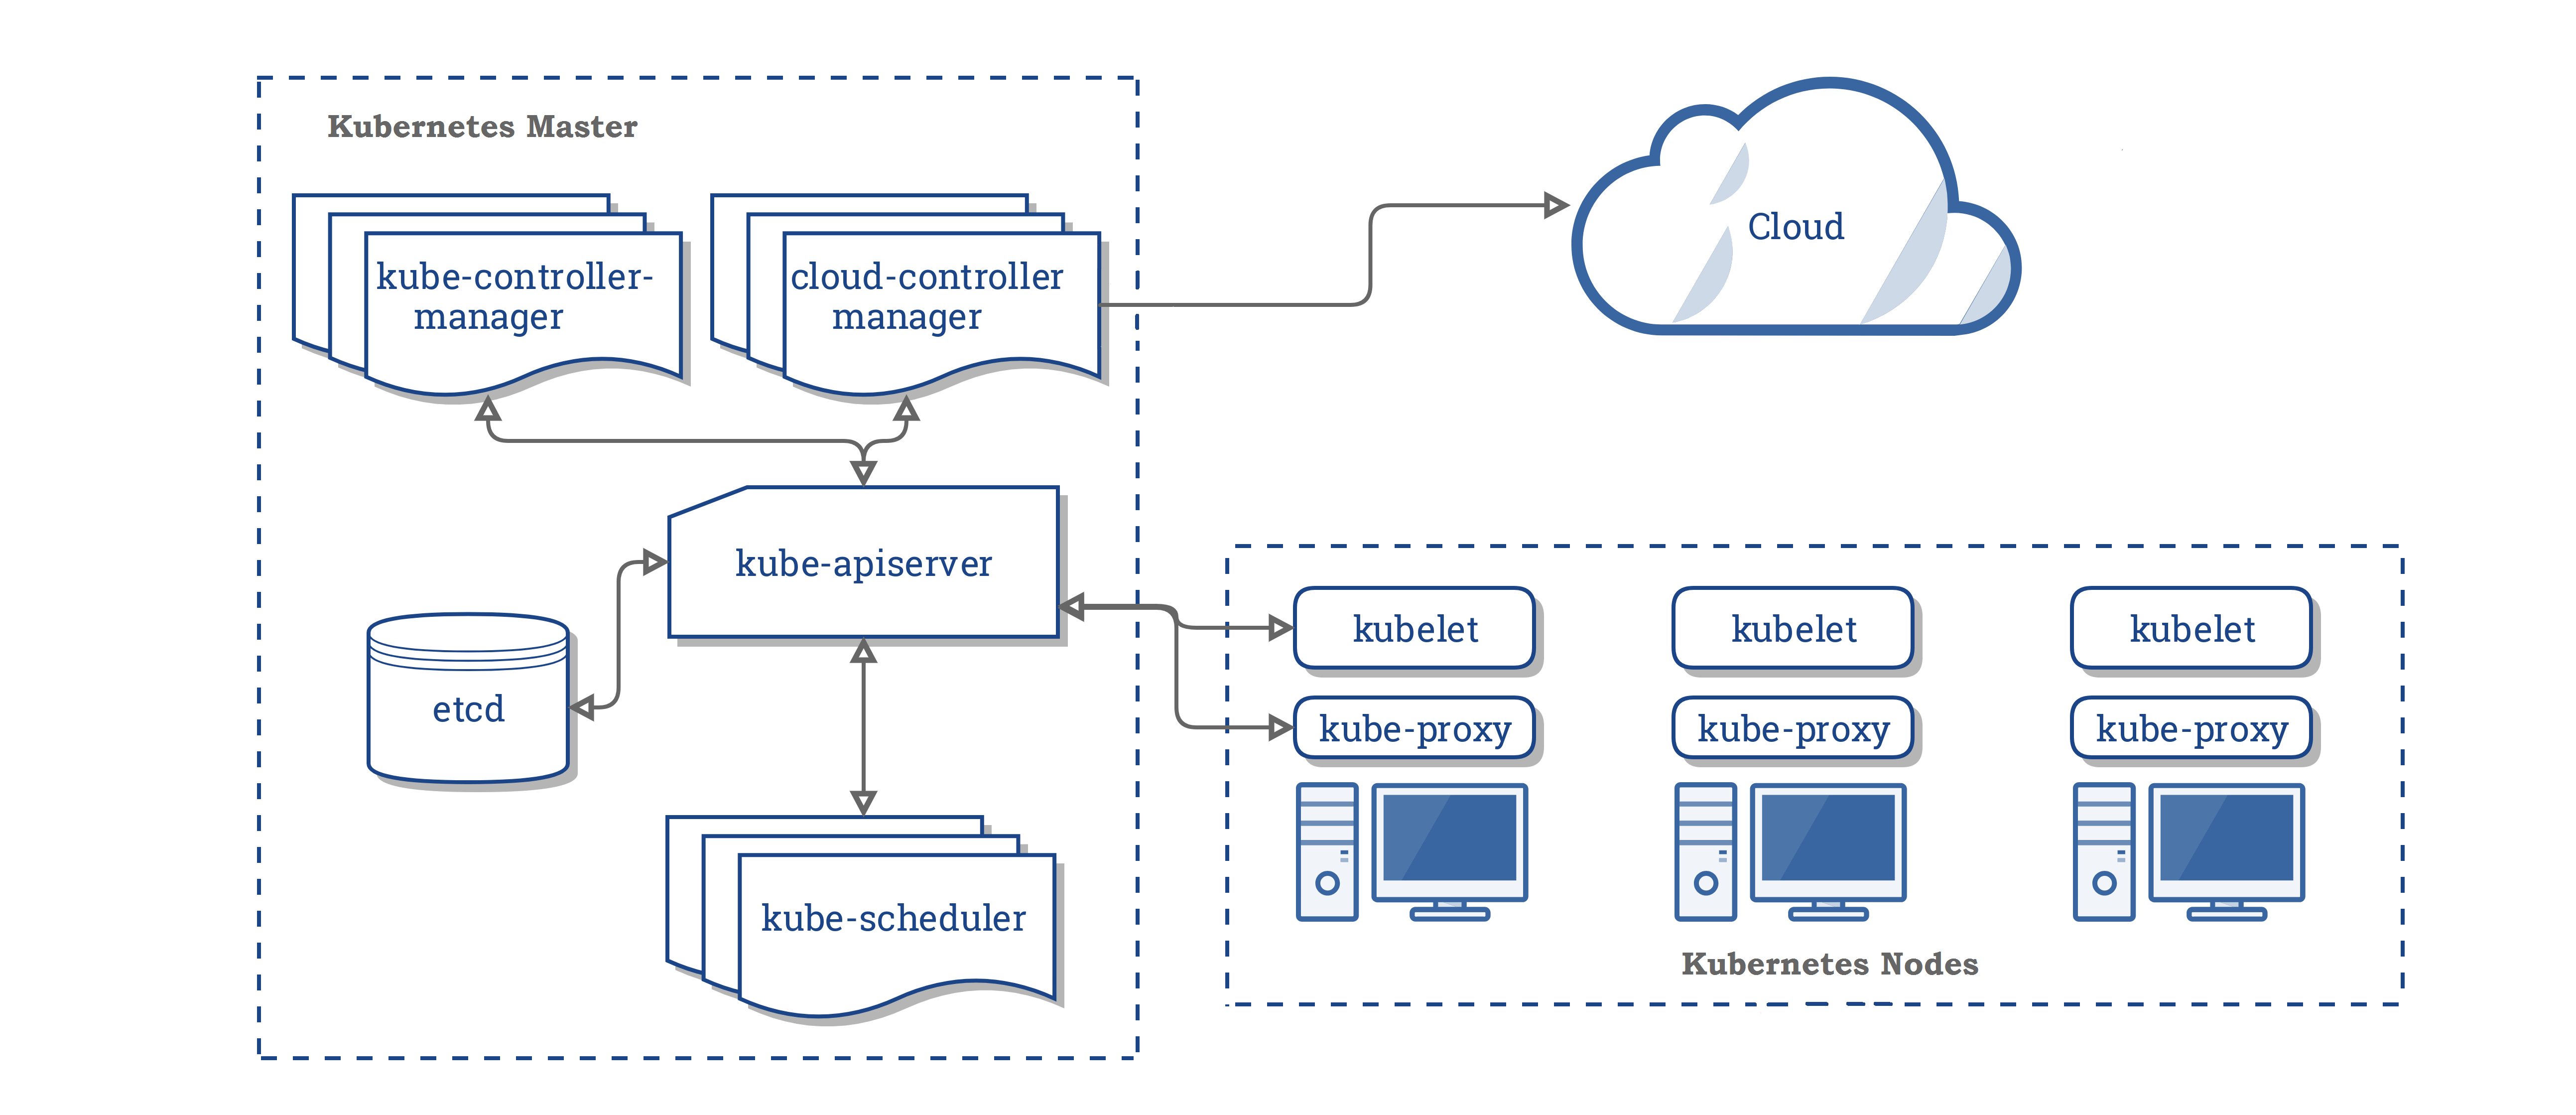
\includegraphics[width=1\linewidth]{images/components-of-kubernetes}
	\caption{Przykładowy klaster wraz z komponentami \cite{kube_doku}.}
	\label{fig:components-of-kubernetes}
\end{figure}

\subsubsection{Master Node}
Jak już wspomniano, master node służy do zarządzania klastrem oraz kontenerami. Podejmuje on decyzje, o umieszczeniu danego poda w node oraz zarządza ich zasobami. Składa się z szeregu komponentów, które zostały wypisane oraz opisane poniżej:
\begin{description}
	\item [kube-apiserver] komponent control plane kubernetesa odpowiedzialny za komunikację użytkownika z platformą. 
	\item [etcd] silnie spójny i wysoce dostępny, rozproszony magazyn w formie klucz-wartość. Zapewnia niezawodny sposób przechowywania konfiguracji kubernetesa. Jeden z ważniejszych komponentów, któremu konieczne jest zapewnienie nadmiarowości. Aby móc tolerować awarię jednego z modułów, konieczne jest stworzenie klastra z ilością trzech.
	\item [kube-scheduler] komponent, który w momencie wykrycia utworzenia nowego poda przypisuje go do odpowiedniego node bądź wielu. Decyzje te podejmuje na podstawie wymagań dotyczących zasobów/sieci poda oraz obciążenia obecnych workerów w klastrze. 
	\item [kube-controller-manager] komponent służący do uruchamiania kontrolerów. (https://kubernetes.io/docs/concepts/architecture/controller/) Każdy z kontrolerów jest osobnym procesem, lecz aby zwiększyć wydajność kompilowane są do jednego pliku binarnego. Zarządza on następującymi kontrolerami:
	\item [node controller] odpowiada za reakcje, w momencie awarii jednego z node.
	\item [replication controller] zapewnia nadmiarowość podów w klastrze.
	\item [endpoints controller] zapewnia spójność usług oraz podów
	\item [service account and token controllers] tworzy użytkowników oraz zapewnia dostęp do API.
	\item [cloud-controller-manager] zapewnia integrację z siecią dostawcy usług chmurowych. 
\end{description}

\subsubsection{Node}
Poza kluczowymi komponentami wymienionymi w rozdziale wyżej, które występują tylko w master node, istnieją również dwa uruchamiane także na worker node.
\begin{itemize}
	\item kubelet - komponent, którego zadaniem jest uruchamianie kontenerów wewnątrz podów. 
	\item kube-proxy - zarządza regułami sieciowymi w node, pozwalającymi na komunikację podów z zasobami wewnątrz oraz poza klastrem. Jeżeli jest taka możliwość,` używa on zasoby oraz mechanizmy filtracji pakietów hosta.
	\item Container Runtime - komponent uruchamiający kontenery w klastrze. Na przykład: Docker, Containerd cri-o, bądź inny wspierany.
\end{itemize}



\section{Calico}
Calico jest to oprogramowanie wykorzystywane do zapewnienia sieci oraz jej bezpieczeństwa w środowiskach zwirtualizowanych i skonteneryzowanych. Jest ono otwarte i może być wykorzystywane przez wiele systemów takich jak OpenStack, OpenShift, Docker EE oraz Kubernetes. Głównymi założeniami twórców było stworzenie systemu skalowalnego w środowiskach opartych o rozwiązania chmurowe. Ponadto, kluczowym aspektem było zapewnienie wydajności zbliżonej do rozwiązań oparty o jądro linuxa. Największymi zaletami Calico są:
\begin{itemize}
	\item Bezpieczeństwo - Użycie modelu “zero trust network” - wszystko co nie jest dozwolone, jest zakazane.
	\item Wydajność - Calico korzysta z wbudowanych w jądro linuxa, wysoko zoptymalizowanych rozwiązań przekazywania oraz filtracji pakietów. W większości przypadków, zbędne jest użycie funkcji enkapsulujących oraz dekapsulujących.
	\item Skalowalność - Osiągnięto ją, dzięki wykorzystaniu najlepszych wzorców projektowych dla środowisk zwirtualizowanych oraz najpopularniejszych i najlepiej sprawdzonych protokołów sieciowych. Calico w cyklu testów deweloperskich jest uruchamiane na klastrze posiadającym wiele tysięcy node’s. 
	\item Uniwersalność - Poza zapewnieniem sieci dla systemów takich jak Kubernetes, możliwe jest również wykorzystywanie w klasycznych maszynach wirtualnych, a także interfejsach fizycznych.
\end{itemize}
\subsection{Host endpoints}
Calico poza możliwością definiowania punktów końcowych dla podów, maszyn wirtualnych, bądź kontenerów umożliwia również tworzenie endpoints dla fizycznych interfejsów. Tak samo host endpoints może zawierać etykiety, które zna-dują się w tej samej przestrzeni nazw co workload endpoints. Calico nie wspiera konfiguracji adresów IP, bądź konfiguracji w oparciu na adresach MAC interfejsów. Konieczna jest zatem ich konfiguracja przez sieć podkładową naszego systemu.

Calico rozróżnia workload endpoints od host endpoints, za pomocą konfigurowalnych prefiksów. Dzięki polu InterfacePrefix w konfiguracji modułu Felix możemy zdecydować, że punkty końcowe zaczynające się od danej wartości będą traktowane jako interfejsy workload. Pozostałe natomiast, będą oznaczać interfejsy hosta.

Calico domyślnie blokuje cały ruch między workload interfaces, pozwalając tylko na ruch, gdy interfejs jest znany oraz skonfigurowane są reguły bezpieczeństwa. W przypadku host endpoints, Calico jest bardziej pobłażliwe. Monitoruje tylko ruch między zdefiniowanymi interfejsami, natomiast nie analizuje wszelkiego innego.

Możemy zastosować reguły bezpieczeństwa, w kontekście punktów końcowych hosta dla trzech rodzajów ruchu:
\begin{itemize}
	\item zakończonego lokalnie,
	\item przekazywanego między host endpoints
	\item przekazywanego pomiędzy host endpoint a workload endpoint.
\end{itemize}
Przykład zastosowania wszystkich trzech rodzajów ruchu, zaprezentowano na grafice poniżej;

\begin{figure}[h!]
	\centering
	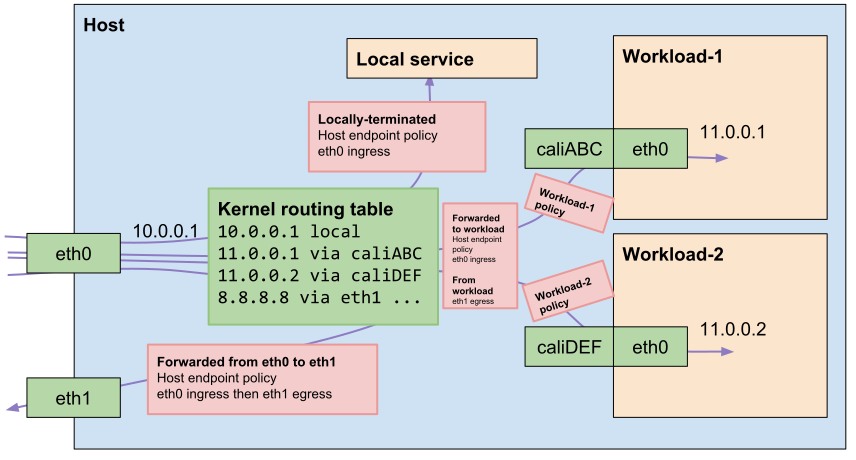
\includegraphics[width=1\linewidth]{images/bare-metal-packet-flows}
	\caption{Schmat pokazujący działanie calico w kontekście host endpoints \cite{calico_doku}.}
	\label{fig:bare-metal-packet-flows}
\end{figure}


\chapter{Uruchomienie klastra}
W celu realizacji pracy magisterskiej, stworzono klaster Kubernetes’a składający się z 6 node. W celu symulacji maszyn fizycznych, wykorzystano narzędzie KVM. Każdy z node, to osobna maszyna wirtualna,  połączona ze sobą przy pomocy sieci izolowanej. Dodatkowo, każdy z node posiada adres publiczny, w celu zapewnienia dostępu do internetu. Systemem operacyjnym dla node jest Ubuntu 18.04.3 LTS. Reasumując, wykorzystano maszyny wirtualne zgodnie z tabelą \ref{tab:kvm_node}.

\begin{table}[h!]
	\begin{tabular}{lllllllll}
		Nazwa hosta   & Adres IP lokalny & Adres IP publiczny &  &  & CPU    & RAM  & Dysk &  \\
		k8s-01-master & 10.10.1.1        & 212.127.89.81     &  &  & 4 Core & 4 GB & 40GB &  \\
		k8s-02-master & 10.10.1.2        & 212.127.89.82     &  &  & 4 Core & 4 GB & 40GB &  \\
		k8s-03-master & 10.10.1.3        & 212.127.89.83     &  &  & 4 Core & 4 GB & 40GB &  \\
		k8s-04-worker & 10.10.1.4        & 212.127.89.84     &  &  & 2 Core & 2 GB & 40GB &  \\
		k8s-05-worker & 10.10.1.5        & 212.127.89.85     &  &  & 2 Core & 2 GB & 40GB &  \\
		k8s-06-worker & 10.10.1.6        & 212.127.89.86     &  &  & 2 Core & 2 GB & 40GB & 
	\end{tabular}
	\label{tab:kvm_node}
	\caption{Lista node klastra}
\end{table}
Wykorzystanie trzech master node wymusza użycie loadbalancera. Do tego celu wykorzystano kolejną maszynę wirtualną z zainstalowanym HAProxy. Konfiguracja ta pozwala na awarię jednego master node oraz dwóch worker node bez wpływu na działanie klastra.

W celu uruchomienia klastra wykorzystano narzędzie kubeadm wspierające nas w jego tworzeniu. Dzięki temu, uruchomienie Kubernetesa staje się szybsze bez uszczerbku na wydajności. Dużym atutem tego narzędzia, jest możliwość bardzo szybkiego dodania kolejnego worker node w razie potrzeby. Kolejne kluczowe kroki, wraz z komendami zostały opisane poniżej.


\section{Loadbalancer}
Jako loadbalancer użyto narzędzia HAProxy zainstalowanego na maszynie wirtualnej o poniższych parametrach:
\begin{table}[h!]
	\begin{tabular}{lllllllll}
		Nazwa hosta   & Adres IP lokalny & Adres IP publiczny &  &  & CPU    & RAM  & Dysk &  \\
		k8s-loadbalancer & 10.10.1.100        & Brak     &  &  & 2 Core & 2 GB & 40GB & 
	\end{tabular}
	\label{tab:kvm_lb}
	\caption{Parametry loadbalancer'a.}
\end{table}
Pakiet haproxy znajduje się w repozytorium, zatem:
\begin{lstlisting}[language=Bash]
sudo apt install haproxy
\end{lstlisting}
Następnie należy skonfigurować loadbalancer za pomocą pliku \textit{haproxy.cfg} w katalogu \textit{/etc/haproxy/}. Zawartość pliku konfiguracyjnego znajduje się poniżej.

\begin{lstlisting}[language=Bash]
frontend kubernetes
bind 10.10.1.100:6443
option tcplog
mode tcp
default_backend kubernetes-master

backend kubernetes-master
mode tcp
balance roundrobin
option tcp-check
server k8s-01-master 10.10.1.1:6443 check fall 3 rise 2
server k8s-02-master 10.10.1.2:6443 check fall 3 rise 2
server k8s-03-master 10.10.1.3:6443 check fall 3 rise 2
\end{lstlisting}


\section{Wyłączenie nftables}
Kubernetes wykorzystuje iptables i jest przygotowany do pracy z tym modułem. Najnowsze dystrybucje takie jak Debian Buster, Ubuntu 19.04, Fedora 29 wykorzystują nowsze narzędzie nftables. Należy pamiętać, aby iptables nie wykorzystywało nftables jako backend. W przypadku wykorzystania Ubuntu 18.04.03 LTS można ten krok pominąć, jednak warto mieć to na uwadze.
\begin{lstlisting}[language=Bash]
sudo -i
update-alternatives --set iptables /usr/sbin/iptables-legacy
update-alternatives --set ip6tables /usr/sbin/ip6tables-legacy
update-alternatives --set arptables /usr/sbin/arptables-legacy
update-alternatives --set ebtables /usr/sbin/ebtables-legacy
\end{lstlisting}

\section{Aktualizacja systemu oraz instalacja niezbędnych paczek}
Przed instalacją pakietów, konieczna jest aktualizacja systemu oraz dodanie repozytorium Kubernetesa.
\begin{lstlisting}[language=Bash]
sudo -i
apt-get update && apt upgrade -y
apt-get install -y apt-transport-https ca-certificates curl software-properties-common
curl -s https://packages.cloud.google.com/apt/doc/apt-key.gpg | sudo apt-key add -
cat <<EOF | sudo tee /etc/apt/sources.list.d/kubernetes.list
deb https://apt.kubernetes.io/ kubernetes-xenial main
EOF
apt-get update
\end{lstlisting}

Następnie należy zainstalować system kontenerów, czyli Docker. Wersja Kubernetesa 1.17 wymaga go w maksymalnie wersji 19.03 i taka też zostanie zainstalowana. Warto pamiętać, o blokadzie automatycznej aktualizacji w celu zapewnienia stabilności klastra.

\begin{lstlisting}[language=Bash]
sudo -i
curl -fsSL https://download.docker.com/linux/ubuntu/gpg | apt-key add -
cat <<EOF | sudo tee /etc/apt/sources.list.d/docker.list
deb https://download.docker.com/linux/ubuntu bionic stable
EOF
apt-get update && apt-get install -y \
docker-ce=5:19.03.4~3-0~ubuntu-$(lsb_release -cs) \
docker-ce-cli=5:19.03.4~3-0~ubuntu-$(lsb_release -cs)
apt-mark hold docker-ce docker-ce-cli
\end{lstlisting}	
Po instalacji Docker'a należy zmienić domyślny sterownik cgroup z cgroupfs, na rekomendowany systemd. 
\begin{lstlisting}[language=Bash]
sudo -i
cat > /etc/docker/daemon.json <<EOF
{
"exec-opts": ["native.cgroupdriver=systemd"],
"log-driver": "json-file",
"log-opts": {
"max-size": "100m"
},
"storage-driver": "overlay2"
}
EOF

mkdir -p /etc/systemd/system/docker.service.d

systemctl daemon-reload
systemctl restart docker
\end{lstlisting}
Ostatnim krokiem jest instalacja kubeadm oraz pakietów Kubernetesa. Przed jego uruchomieniem, konieczne jest wyłączenie partycji SWAP.
\begin{lstlisting}[language=Bash]
sudo apt-get install -y kubelet kubeadm kubectl
sudo apt-mark hold kubelet kubeadm kubectl
\end{lstlisting}

\section{Stworzenie master oraz worker node}
Jak już wspomniano, do instalacji klastra wykorzystano narzędzie kubeadm, pozwalające przyśpieszyć wiele procesów instalacyjnych. Najważniejszymi poleceniami wspomnianej aplikacji, jest kubeadm init oraz kubeadm join. Najpierw zostało opisane polecenie inicjalizujące control plane klastra tj. kubeadm init. Posiada ono, szereg argumentów pozwalających na dostosowanie klastra do własnych potrzeb. Najważniejsze opisano poniżej:
\begin{description}
	\item[control-plane-endpoint] Przydatne szczególnie, w komecie rozbudowy klastra o kolejny master node. Umożliwia ustawienie wspólnego punktu końcowego, dla wszystkich węzłów control plane.
	\item[pod-network-cidr] Określa pulę adresów IP, wykorzystywanych dla sieci z podami.
	\item[apiserver-advertise-address] Domyślnie kubeadm używa interfejsu przypisane do bramy domyślnej jako adresu docelowego serwera API master node.
	\item[upload-certs] Opcja ta pozwala na wysłanie potrzebnych certyfikatów do bazy kubeadm.
\end{description}
Zatem, polecenie inicjalizujące pierwszy control plane klastra to: 
\begin{lstlisting}[language=Bash]
kubeadm init --control-plane-endpoint 10.10.1.100 --pod-network-cidr 192.168.0.0/18 --apiserver-advertise-address 10.10.1.100 --upload-certs
\end{lstlisting}
Jeżeli wszystko zostanie sprawnie zainstalowane, będziemy o tym poinformowani stosownym komunikatem. Zawiera on również informację o możliwości dodania kolejnego node. Jego fragment został zaprezentowany poniżej:

\begin{lstlisting}[language=Bash]
Your Kubernetes control-plane has initialized successfully!

To start using your cluster, you need to run the following as a regular user:

mkdir -p $HOME/.kube
sudo cp -i /etc/kubernetes/admin.conf $HOME/.kube/config
sudo chown $(id -u):$(id -g) $HOME/.kube/config

You can now join any number of control-plane nodes by copying certificate authorities
and service account keys on each node and then running the following as root:

kubeadm join 10.10.1.100:6443 --token xx.xxx \
--discovery-token-ca-cert-hash sha256:xxxx \
--control-plane 

Then you can join any number of worker nodes by running the following on each as root:

kubeadm join 10.10.1.100:6443 --token xx.xxx \
--discovery-token-ca-cert-hash sha256:xxxx
\end{lstlisting}


Dodajemy kolejno dwa master node oraz trzy worker node. Dzięki wykorzystaniu kubeadm możliwe jest to za pomocą jednego polecenia, odpowiednio z flagą \textit{--control-plane} dla master node, bądź bez.
\begin{lstlisting}{language=Bash}
kubeadm join 10.10.1.100:6443 --token xx.xxx --discovery-token-ca-cert-hash sha256:xxxx
\end{lstlisting}
W przypadku braku tokenu, możliwe jest jego stworzenie wykonując poniższe polecenie na master node:
\begin{lstlisting}[language=Bash]
kubeadm token create
\end{lstlisting}
natomiast hash certyfikatu zostanie wyświetlony poleceniem:
\begin{lstlisting}[language=Bash]
openssl x509 -pubkey -in /etc/kubernetes/pki/ca.crt | openssl rsa -pubin -outform der 2>/dev/null \
| openssl dgst -sha256 -hex | sed 's/^.* //'
\end{lstlisting}

Gotowość klastra możemy zweryfikować poprzez wypisanie działających node.

\begin{lstlisting}[language=Bash]
rdziwinski@k8s-01-master:~$ kubectl get node
NAME            STATUS     ROLES    AGE     VERSION
k8s-01-master   Ready      master   7d21h   v1.17.2
k8s-02-master   Ready      master   7d23h   v1.17.2
k8s-03-master   Ready      master   7d23h   v1.17.2
k8s-04-worker   Ready      <none>   7d22h   v1.17.2
k8s-05-worker   Ready      <none>   7d22h   v1.17.2
k8s-06-worker   Ready      <none>   7d22h   v1.17.2

\end{lstlisting}


Master i worker node są gotowe do pracy. Kolejnym krokiem jest ręczne przypisanie adresu IP dla każdego z node. W tym celu, na każdym z node należy edytować plik konfiguracyjny dodając argument --node-ip=10.10.1.x do zmiennej KUBELET\_CONFIG\_ARGS:
\begin{lstlisting}[language=Bash]
vim /etc/systemd/system/kubelet.service.d/10-kubeadm.conf
\end{lstlisting}
oraz zresetować procesy
\begin{lstlisting}[language=Bash]
systemctl daemon-reload
systemctl restart kubelet
\end{lstlisting}

\section{Calico}
Jak już wspomniano, do zapewnienia sieci wewnątrz klastra wykorzystano narzędzie Calico. Instalacja jego odbywa kolejno w trzech krokach: 

\begin{enumerate}
	\item Pobranie pliku konfiguracyjnego ze strony: \\ \textit{https://docs.projectcalico.org/v3.11/manifests/calico.yaml}
	\item Edycja wartości \textit{CALICO\_IPV4POOL\_CIDR} zgodnie z zadeklarowaną wcześniej pulą.
	\item Wykonanie pliku konfiguracyjnego. \textit{kubectl apply -f calico.yaml}
\end{enumerate}

Poprawną instalację możemy zweryfikować poprzez sprawdzenie obecności podów wykorzystywanych przez system calico. Jeżeli wszystko jest poprawne powinniśmy zobaczyć informacje jak poniżej:
\begin{lstlisting}[language=Bash]
rdziwinski@k8s-01-master:~$ kubectl get pods -n kube-system
NAME                                       READY   STATUS    RESTARTS   AGE
calico-kube-controllers-5b644bc49c-zdhqn   1/1     Running   227        3d21h
calico-node-5hcfb                          1/1     Running   4          3d21h
calico-node-8d7h2                          1/1     Running   9          3d21h
calico-node-dwrjp                          1/1     Running   9          3d21h
calico-node-ghtkc                          1/1     Running   4          3d21h
calico-node-mtkkx                          1/1     Running   4          3d21h
calico-node-nqpgl                          1/1     Running   9          3d21h
coredns-6955765f44-2r7ch                   1/1     Running   5          3d21h
coredns-6955765f44-gm2b5                   1/1     Running   3          3d22h
etcd-k8s-01-master                         1/1     Running   28         7d22h
etcd-k8s-02-master                         1/1     Running   39         7d23h
etcd-k8s-03-master                         1/1     Running   29         7d23h
kube-apiserver-k8s-01-master               1/1     Running   55         7d22h
kube-apiserver-k8s-02-master               1/1     Running   45         7d23h
kube-apiserver-k8s-03-master               1/1     Running   45         7d23h
kube-controller-manager-k8s-01-master      1/1     Running   39         7d22h
kube-controller-manager-k8s-02-master      1/1     Running   43         7d23h
kube-controller-manager-k8s-03-master      1/1     Running   33         7d23h
kube-proxy-5sxq5                           1/1     Running   9          7d22h
kube-proxy-7mv2f                           1/1     Running   10         7d23h
kube-proxy-c26tt                           1/1     Running   9          7d22h
kube-proxy-gn72z                           1/1     Running   11         7d23h
kube-proxy-hkfcb                           1/1     Running   9          7d23h
kube-proxy-mm5lh                           1/1     Running   14         7d23h
kube-scheduler-k8s-01-master               1/1     Running   44         7d22h
kube-scheduler-k8s-02-master               1/1     Running   36         7d23h
kube-scheduler-k8s-03-master               1/1     Running   33         7d23h
\end{lstlisting}

Aby móc pracować z calico konieczne jest zainstalowanie narzędzia calicoctl. Aby to zrobić należy pobrać plik binarny z repozytorium calico w serwisie github oaz skopiować do właściwego katalogu.
\begin{enumerate}
	\item curl -O -L  https://github.com/projectcalico/calicoctl/releases/download/v3.11.2/calicoctl
	\item chmod +x calicoctl
	\item sudo cp calicoctl /usr/local/bin/
\end{enumerate}
Ostatnim etapem jest wskazanie calicoctl lokalizacji etcd. Można to zrobić na wiele sposobów, na przykład dopisując poniższe linie do pliku \textit{ ~/.bashrc}:
\begin{lstlisting}[language=Bash]
export KUBECONFIG=/home/rdziwinski/.kube/config
export DATASTORE_TYPE=kubernetes
\end{lstlisting}

Aby uniknąć błędów w czasie pracy z klastrem, gdzie każdy z node ma kilka interfejsów sieciowych należy na stałe ustalić adres IP dla każdego z nich. Aby to zrobić, stworzono plik konfiguracyjny \textit{nodes.yaml} w którym powielono poniższą konfiguracje dla każdego z node zmieniając jedynie wartość \textit{ipv4Address}.
\begin{lstlisting}[language=Bash]
apiVersion: projectcalico.org/v3
kind: Node
metadata:
  name: k8s-01-master
spec:
  bgp:
    ipv4Address: 10.10.1.1/24
\end{lstlisting}
Konfigurację zatwierdzamy poleceniem \textit{calicoctl apply -f nodes.yaml}.



\chapter{Założenia oraz ich realizacja.}


W ramach pracy stworzono projekt sieci firmowej w jednym z oddziałów. Kierowano się następującymi założeniami:
\begin{enumerate}

	\item Każda z placówek posiada 3 sieci wewnętrzne:
	\begin{itemize}
		\item Dział techniczny
		\item Pozostali pracownicy
		\item DMZ
	\end{itemize}

	\item W sieci dla pracowników zostanie uruchomiony serwer DHCP.
	\item Izolacja urządzeń pomiędzy siecią działu technicznego a innych pracowników. Administratorzy powinni posiadać dostęp do urządzeń pracowników.
	\item W DMZ będą znajdować się serwery www. Dwa z nich jako pody a jeden postawiony będzie jako osobna maszyna wirtualna.
	\item Stworzony zostanie pod z instancją routera bird, wykorzystany do wymiany prefixów. W ramach pracy przyjęto, że adresacja rozgłaszana przez nasza firmę to 172.16.0.0/14, natmiast otrzymywana to 172.20.0.0/14. 
\end{enumerate}
Sieć firmową zasymulowano przy pomocy maszyn wirtualnych KVM. Klaster składa się z trzech master node oraz trzech worker nodów. Dodatkowo wykorzystano maszyny wirtualne jako komputery pracowników działu, loadbalancer oraz router z aplikacją Bird. Każdy z node posiada minimum dwa interfejsy:
\begin{itemize}
	\item enp1s0 - adres prywatny z puli 10.10.1.0/24 służący do zarządzania oraz komunikacji między nodami.
	\item eth6s0 - adres publiczny używany jako wyjście na świat.
\end{itemize}
Dodatkowo wszystkie trzy worker node posiadają interfejsy służące do wymiany ruchu między siecią fizyczną firm.


\section{Sieci wewnętrzne}
Sieć firmową podzielono na 3 podsieci wewnętrzne.
\begin{table}[]
	\begin{tabular}{lll}
		Nazwa sieci          & Adresacja       & Interfejs \\
		DMZ                  & 192.168.64.0/22 & enp7s0    \\
		Sieć pracowników     & 192.168.68.0/22 & enp8s0    \\
		Sieć Administratorów & 192.168.72.0/22 & enp9s0   
	\end{tabular}
	\label{tab:adresacje}
	\caption{Sieci wewnętrzne w firmie.}
\end{table}

\subsection{HostEndpoints}
Jak już wspomniano Calico wykorzystuje zasób hostendpoints aby zdefiniować punkty końcowe sieci fizycznej. W tym celu należy stworzyć osobny zasób dla każdego z interfejsu fizycznego node, wykorzystywanego do działania sieci fizycznej. Poniżej przedstawiono fragment pliku konfiguracyjnego dla interfejsu wykorzystywanego przez pracowników.

\begin{lstlisting}[language=Bash]
apiVersion: projectcalico.org/v3
kind: HostEndpoint
metadata:
  name: k8s-06-enp8s0
  labels: 
    interface: enp8s0
    subnet: pracownicy
spec:
  interfaceName: enp8s0
  node: k8s-06-worker
\end{lstlisting}
Warto zwrócić uwagę na etykietę \textit{subnet} dzięki której jesteśmy w stanie pogrupować interfejsy w zależności od przeznaczenia. Dla zakończeń sieci używanych w przypadku ruchu publicznego, ze względów bezpieczeństwa, oraz wygody konfiguracji użyto innych etykiet. Poniżej znajduje się treść jednego z trzech takich zasobów.
\begin{lstlisting}[language=Bash]
apiVersion: projectcalico.org/v3
kind: HostEndpoint
metadata:
  name: k8s-04-enp6s0
  labels: 
    interface: public
spec:
  interfaceName: enp6s0
  node: k8s-04-worker
\end{lstlisting}

\subsection{Firewall}
Jako narzędzie do separacji ruchu użyto mechanizmu Calico nazwanego GlobalNetworkPolicy. Konfiguracja różni się znacząco od tworzenia reguł w jednym z popularnych narzędzi typu firewall, jednak funkcja jego jest identyczna. Zgodnie z najlepszymi praktykami tworzenia wszelkich reguł bezpieczeństwa zaczęto od blokady każdego ruchu w klastrze.
\begin{lstlisting}[language=Bash]
apiVersion: projectcalico.org/v3
kind: GlobalNetworkPolicy
metadata:
  name: deny-all
spec:
  order: 999
  selector: has(subnet) #1
  applyOnForward: true #2
  types:
  - Ingress
  - Egress
  ingress:
  - action: Deny
  egress:
  - action: Deny
\end{lstlisting}
Kluczowe są dwa parametry:
\begin{enumerate}
	\item linijka ta oznacza, że reguła dotyczy tylko obiektów które posiadają parametr \textit{subnet}, tak jak stworzone wcześniej \textit{hostendpoints}. Takie rozwiązanie zostało wdrożone aby nie zakłócić pracy innych elementów klastra.
	\item dzięki ustawieniu zmiennej applyOnForward na true możliwe jest analizowanie ruchu który przechodzi przez wskazany \textit{hostendpoints}. W przypadku pozostawienia tej wartości jako domyślnej Calico zastosowałoby tworzoną regułę tylko dla ruchu wychodzącego bądź docelowego do tego interfejsu.
\end{enumerate}
W dalszej części pliku konfiguracyjnego blokowany jest ruch przychodzący oraz wychodzący dla odpowiednich zakończeń sieci.

Aby umożliwić łatwiejsze zarządzanie adresacją w sieci stworzone zostały obiekt GlobalNetworkSet. Chcąc porównać do standardowych narzędzi tylu firewall, można powiedzieć, że jest to lista adresów. Fragment pliku konfiguracyjnego został zaprezentowany poniżej:

\begin{lstlisting}[language=Bash]
apiVersion: projectcalico.org/v3
kind: GlobalNetworkSet
metadata:
  name: administratorzy
  labels:
    pool: administratorzy
spec:
  nets:
  - 192.168.72.0/22
\end{lstlisting}

Jednym z założeń sieci firmowej, pokazujące możliwości Calico, było umożliwienie dostępu z sieci administratorów do sieci pozostałych pracowników. W tym celu stworzono kolejny plik konfiguracyjny wraz z regułą \textit{GlobalNetworkPolicy} której którego zawartość znajduje się poniżej:

\begin{lstlisting}[language=Bash]
apiVersion: projectcalico.org/v3
kind: GlobalNetworkPolicy
metadata:
  name: allow-admins
spec:
  order: 4
  selector: subnet in {'administratorzy','pracownicy'} #1
  applyOnForward: true
  types:
  - Ingress
  - Egress
  ingress:
  - action: Allow #2
    protocol: ICMP
    source:
      selector: pool == 'administratorzy'
    destination:
      selector: pool == 'pracownicy'

  - action: Allow #3
    protocol: TCP
    source:
      selector: pool == 'administratorzy'
    destination:
      selector: pool == 'pracownicy'
    ports:
    - [55222,22]    
     egress:
    - action: Allow
\end{lstlisting}
Warto zwrócić uwagę na wyszczególnione linie konfiguracji.
\begin{enumerate}
	\item W tej linii następuje wybór interfejsów na które tworzona reguła będzie wpływać. Zatem wybieramy interfejsy do których podłączone będą urządzenia sieci dla administratorów oraz pozostałych pracowników.
	\item Sekcja ta zezwala na ruch protokołu ICMP, gdzie źródłowy IP należy do sieci administratorzy a docelowy do sieci pracowników.
	\item Analogicznie jak wyżej, jednak w tym przypadku wybieramy protokół TCP oraz porty 55222 i 22. Port 55222 jest portem ssh na którym wystawiony jest komputer w sieci pracowników.
\end{enumerate}

\subsection{Dostęp do internetu}
Aby każda z sieci posiadała dostęp do internetu konieczne jest stworzenie zasobu Calico o nazwie ippool dla każdej z podsieci. Przykładowy plik konfiguracyjny dla sieci administratorów został zaprezentowany poniżej. 

\begin{lstlisting}[language=Bash]
apiVersion: projectcalico.org/v3
kind: IPPool
metadata:
  name: administratorzy
  labels:
    subnet: administratorzy
spec:
  cidr: 192.168.72.0/22
  natOutgoing: true
\end{lstlisting}

Kluczowa w tej konfiguracji jest opcja \textit{natOutgoing} której ustawienie na wartość \textit{true} zezwala na natowanie adresu IP sieci lokalnej na adres publiczny.

Aby ruch wychodzący do internetu oraz przychodzący nie był blokowany należy dodatkowo utworzyć regułę na to zezwalającą. Jej treść znajduje się poniżej.
\begin{lstlisting}[language=Bash]
apiVersion: projectcalico.org/v3
kind: GlobalNetworkPolicy
metadata:
  name: internet
spec:
  order: 20
  selector: subnet in {'pracownicy','administratorzy'}
  applyOnForward: true
  types:
  - Ingress
  - Egress
  ingress:
  - action: Allow
    destination:
      notSelector: pool == 'local'
  egress:
  - action: Allow
    destination:
      selector: interface == 'public'

\end{lstlisting}
Działanie reguły bezpieczeństwa polega na umożliwieniu ruchu wychodzącego do \textit{hostendpoints}, o nazwie internet, z publicznym adresem IP. Jednocześnie zezwalam na ruch przychodzący od sieci innych niż prywatne. Stworzenie takiej reguły zostało wsparte zasobem \textit{globalnetworkset} którego treść znajduje się poniżej. 
\begin{lstlisting}[language=Bash]
apiVersion: projectcalico.org/v3
kind: GlobalNetworkSet
metadata:
  name: local
  labels:
    pool: local
spec:
  nets:
  - 192.168.0.0/16
  - 172.16.0.0/12
  - 10.0.0.0/8
\end{lstlisting}

\subsection{Blokada SSH}
Możliwe jest również wykorzystanie Calico do ograniczenia dostępu bezpośrednio do klastra. Na przykład możemy zablokować logowanie przez ssh. W tym celu stworzono plik konfiguracyjny którego zawartość znajduje się poniżej:

\begin{lstlisting}[language=Bash]
apiVersion: projectcalico.org/v3
kind: GlobalNetworkPolicy
metadata:
name: cluster
spec:
  order: 16
  selector: interface == 'public'
  types:
  - Ingress
  - Egress
  ingress:
  - action: Allow
  - action: Deny
    protocol: TCP
    destination:
      ports: [55222,22]
  egress:
  - action: Allow
\end{lstlisting}

\subsection{DHCP}

W celu umożliwienia wygodnego korzystania z sieci, w podsieci dla pracowników uruchomiono serwer dhcp w postaci aplikacji \textit{isc-dhcpd}. Zgodnie z założeniem uruchamiania usług wykorzystując kontenery i pody stworzono dwa pliki konfiguracyjne. Pierwszy z nich tworzy obiekt typu \textit{DaemonSet}, natomiast drugi \textit{ConfigMap}. Treść pierwszego z nich, wraz z komentarzem przedstawiono poniżej.

\begin{lstlisting}[language=Bash]
apiVersion: apps/v1
kind: DaemonSet #1
metadata:
  name: dhcpd
  labels:
    app: dhcpd
spec:
  selector:
    matchLabels:
      app: dhcpd
  updateStrategy:
    type: RollingUpdate
  template:
    metadata:
      labels:
        app: dhcpd
    spec:
      hostNetwork: true #2
      containers:
      - name: main
        image: docker.io/pnnlmiscscripts/dhcpd:4.4.1-4 #3
        imagePullPolicy: Always
        command: #4
        - /bin/sh
        - -ec
        - |
        touch /var/lib/dhcp/dhcpd.leases
        chown daemon.daemon /var/lib/dhcp/dhcpd.leases
        chown daemon.daemon /var/lib/dhcp
        chown daemon.daemon /var/run/dhcp
        dhcpd -cf /etc/dhcp/dhcpd.conf -d -user daemon -group daemon enp7s0 enp8s0 enp9s0
      volumeMounts:
      - name: config
        mountPath: /etc/dhcp
    volumes:
    - name: config
      configMap: #5
        name: dhcpd
\end{lstlisting}

\begin{enumerate}
	\item DaemonSet jest to specjalny rodzaj podu który tworzony jest na każdym z dostępnych worker node. 
	\item Konfiguracja ta umożliwia bezpośrednią widoczność serwera DHCP przez fizyczne interfejsy sieciowe node. jest to wymagane ze względu na mechanizm działania protokołu DHCP, który wymaga w standardowej konfiguracji widoczności w warstwie drugiej obu urządzeń.
	\item Przed uruchomieniem aplikacji konieczna jest jej konfiguracja poprzez zmianę uprawnień dla używanych przez nią zasobów dyskowych. Ostatnia linijka bloku \textit{command} uruchamia serwer dhcp dla wskazanych interfejsów.
	\item Konfiguracja serwera nie jest zapisana na stałe w kontenerze a dynamicznie aktualizowana poprzez strukturę \textit{configMap} opisaną w dalszej części.
\end{enumerate}

Drugim z plików konfiguracyjnych jest obiekt \textit{configMap} który umożliwia w prosty sposób wprowadzaniem zmian na wszystkich dostępnych podach na raz. Jego treść znajduje się poniżej.

\begin{lstlisting}[language=Bash]
apiVersion: v1
kind: ConfigMap
metadata:
  name: dhcpd
  labels:
    app: dhcpd
data:
  dhcpd.conf: |
    default-lease-time 600;
    max-lease-time 7200;
    ddns-update-style none;
    subnet 192.168.68.0 netmask 255.255.252.0 {
      range 192.168.68.10 192.168.68.240;
      option routers 192.168.71.254;
      option domain-name-servers 8.8.4.4;
      option subnet-mask 255.255.252.0;
    }
    subnet 192.168.72.0 netmask 255.255.252.0 {
      range 192.168.72.10 192.168.72.240;
      option routers 192.168.75.254;
      option domain-name-servers 8.8.4.4;
      option subnet-mask 255.255.252.0;
    }
\end{lstlisting}

\subsection{Brama domyślna}
Jak można zauważyć, w konfiguracji serwera DHCP brama domyślna została zdefiniowana jako ostatni adres IP z każdej puli, na przykład: 192.168.75.254. Adresacja ta nie jest natomiast skonfigurowana na żadnym z interfejsów. Jest to spowodowane wykorzystaniem protokołu VRRP w celu zapewniania pełniej niezawodności sieci. Jako daemona wspomnianego protokołu wykorzystano aplikację \textit{keepalived} .Konfiguracja jej polega na edycji pliku \textit{keepalived.conf} znajdującego się w katalogu \textit{/etc/keepalived/}. Poniżej zamieszczono przykładową konfigurację dla node \textit{k8s-05-worker}.
\begin{lstlisting}[language=Bash]
global_defs {
	vrrp_skip_check_adv_addr
}

vrrp_instance dmz {
	interface enp7s0          
	state MASTER
	unicast_src_ip 192.168.67.245
	unicast_peer {
		192.168.67.244
		192.168.67.246
	}
	virtual_router_id 64     
	priority 200               
	virtual_ipaddress {
		192.168.67.254/22     
	}
}

vrrp_instance pracownicy {
	interface enp8s0         
	state MASTER   
	unicast_src_ip 192.168.71.245
	unicast_peer {
		192.168.71.244
		192.168.71.246
	}
	
	virtual_router_id 68  
	priority 200             
	virtual_ipaddress {
		192.168.71.254/22   
	}
}

vrrp_instance administratorzy {
	interface enp9s0
	state MASTER          
	unicast_src_ip 192.168.75.245
	unicast_peer {
		192.168.75.244
		192.168.75.246
	}
	virtual_router_id 72      
	priority 200               
	virtual_ipaddress {
		192.168.75.254/22        
	}
}
\end{lstlisting}
Stworzone zostały trzy instancję protokołu VRRP, po jednej dla każdej z podsieci. Konfiguracja dla każdego node jest bardzo zbliżona. Różnicą między nimi jest inna wartość parametru \textit{state} oraz \textit{priority}. Kolejno BACKUP oraz priorytet 100 i 50. Domyślnie protokół VRRP działa w trybie multicast, natomiast wykorzystanie maszyn wirtualnych wymusiło zmianę trybu pracy na unicast. Jest to spowodowane ograniczeniem możliwości przesyłania pakietów multicastowych poprzez interfejsy VTEP w KVM.


\section{Peering z zewnętrznym routerem BGP}


\chapter{Porównanie rozwiązania zwirtualizowanego do fizycznego} w oparciu o przyjęte kryteria.
Obecnie najpopularniejszą formą zapewnienia routingu w sieci jest wykorzystanie klasycznych routerów oraz przełączników sprzętowych. W zależności od wielkości firmy, stosuje się bardzo proste routery domowe, bądź bardziej zaawansowane produkty firm takich jak Cisco bądź Juniper. W przypadku gdy korporacja wymaga zaawansowanego routingu nie tylko dla potrzeb sieci wewnętrznej w jednej placówce, konieczne jest zakup dodatkowych urządzeń. Potrzebne są wtedy wydaje routery BGP bądź Firewalle potrafiące zestawić wydajne tunele VPN. 

Obecnie coraz więcej usług jest realizowanych przez oprogramowanie zainstalowane na serwerach. Fizyczne urządzenia dedykowane pod dany rodzaj usług stają się coraz mniej popularne. W niniejszym rozdziale zostanie poddana analiza zalet oraz wad rozwiązania fizycznego do zwirtualizowanego. Przez pojęcie zwirtualizowanego rozumie się wykorzystanie zyskujących na popularności kontenerów, wraz z Orkiestratorem Kubernetes, oraz siecią realizowaną przez Calico. Kryteria porównawcze które przyjęto to:
\begin{itemize}
	\item uniwersalność
	\item koszt wdrożenia
	\item koszt utrzymania
	\item łatwość konfiguracji
	\item możliwość rozbudowy
\end{itemize}

\section{Uniwersalność}
Routery sprzętowe popularnych producentów obsługują ogromną liczbę protokołów które przez swoje specyficzne wymagania mogą być niedostępne dla rozwiązania zwirtualizowanego. Jednym z takich protokołów jest MPLS, zatem w przypadku konieczności obsługi wspomnianego protokołu zalecany jest wybór rozwiązania fizycznego.

W przypadku analizy uniwersalności, jako możliwość zastosowania sprzętu w wielu dziedzinach zdecydowaną przewagę uzyskują rozwiązania zwirtualizowane. Zakupując router sprzętowy jego funkcjonalność ogranicza się jedynie do sprawowania tej jednej funkcji. Wszelka integracja z systemami wewnętrznymi firmy jest bardzo skomplikowana i czasem niemożliwa. Korzystając z routera którego konfiguracja odbywa się poprzez pliki yaml, tak jak w przypadku opisywanego rozwiązania, istnieje możliwość łatwej integracji z oprogramowaniem firmy. Takim przykładem są wszelkie systemy CRM bądź zarządzania pracownikami. 

Główną przewagą w aspekcie uniwersalności jest możliwość wykorzystania praktycznie dowolnego komputera klasy PC, bądź serwera. W przypadku potrzeby stworzenia sieci wewnątrz firmy możliwe jest zastosowanie nieużywanego już sprzętu bądź zakup nowego. W tym przypadku zakupione urządzenie może również służyć w innych obszarach działalności firmy.

\section{Koszty}
Analiza kosztu zakupu w oparciu o serwis allegro. Ceny podane orientacyjnie, bez konkretnych ofert.
Koszty utrzymania.



\section{Łatwość konfiguracji}
bardzo subiektywne. Pokazanie różnic. Skupienie się na popularności obsługi np. CLI z IOS Cisco oraz małą popularność systemu Kubernetes.
\section{Możliwość rozbudowy}
Duże pole do popisu dla rozwiązań zwirtualizowanych.

\chapter{Procedury testowe}
Jakiś wstęp...

\section{Testy wydajności}
Z powodu ograniczeń technicznych i braku możliwości porównania z podobną platformą sprzętową, testy wydajności zostaną przeprowadzone tylko w środowisku zwirtualizowanym. Podczas testów stworzone będą cztery scenariusze możliwe w czasie pracy firmy.
//Ewentualnie można porównać niektóre testy z komputerem fizycznym wpiętym w ten sam segment sieci.
\begin{enumerate}
	\item Wysyłanie pliku na serwer.
	\item Pomiar średniego czasu odpowiedzi.
	\item Przesyłanie danych między siecią Administratorów a pracowników.
	\item Czas dostępu do strony www w klastrze.
\end{enumerate}
Środowisko testowe, tj. klaster Kubernetes został stworzony jako zespół maszyn wirtualnych. Również komputery pracowników to maszyny wirtualne uruchomione na tym samym komputerze. Jako maszyna supervisor posłużył zmodyfikowany komputer MacPro 4,1 Early 2009. Specyfikacja kluczowych parametrów znajduje się poniżej:
\begin{itemize}
	\item Procesor: 2x Xeon E5520 4 Core 2.26GHz
	\item Pamięć ram: 4x8GB DDR3 1066 MT/s
	\item Karta sieciowa: Intel Corporation 82574L Gigabit Network Connection
	\item Dysk twardy: Samsung HD103SJ 
	\item System Operacyjny: Debian 10	
\end{itemize}

Maszyny wirtualne zostały stworzone przy pomocy rozwiązania KVM oraz QEMU w ich najnowszych wersjach, dostępnych w repozytorium Debian Buster. Poniżej została przedstawiona specyfikacja każdej z VM. W prawej części znajdują się również informacje na temat średniego obciążenia w spoczynku. Przez to pojęcie rozumie się normalną prace klastra wraz z uruchomionymi wszystkimi usługami. Nie są one jednak w żaden sposób wykorzystywane. Procesor w każdej z maszyn wirtualnych emuluje CPU supervisora. Kolumna load oznacza wartość parametru systemu linux \textit{Load Averages} dla ostatnich 15 minut. Na każdej maszynie wirtualnej został zainstalowany system operacyjny Ubuntu 18.04.3 LTS bez środowiska graficznego.

\begin{table}[]
	\begin{tabular}{lccccccc}
		& CPU {[}core{]} & RAM {[}GB{]} & load &  &  &  &  \\
		supervisor       & 16             & 32           & 3.07 &  &  &  &  \\
		k8s-01-master    & 4              & 4            &      &  &  &  &  \\
		k8s-02-master    & 4              & 4            &      &  &  &  &  \\
		k8s-03-master    & 4              & 4            &      &  &  &  &  \\
		k8s-04-worker    & 2              & 2            &      &  &  &  &  \\
		k8s-06-worker    & 2              & 2            &      &  &  &  &  \\
		k8s-05-worker    & 2              & 2            &      &  &  &  &  \\
		k8s-loadbalancer & 2              & 1            &      &  &  &  &  \\
		administratorzy  & 1              & 512          &      &  &  &  &  \\
		pracownicy       & 1              & 512          &      &  &  &  &  \\
		&                &              &      &  &  &  & 
	\end{tabular}
\end{table}

\subsection{Wysyłanie pliku na serwer}
Pierwszy test symuluje wysyłanie dużego pliku na zewnętrzny serwer w internecie. Do tego celu wykorzystano narzędzie iperf3. Pomiar został wykonany do serwera umieszczonego w obrębie sieci lokalnej, do którego minimalna przepustowość łącza wynosi 1Gbps. Klienta uruchomiono na maszynie wirtualnej \textit{pracownicy}. Parametry testu są następujące:
\begin{itemize}
	\item Czas trwania: 30 sekund.
	\item Serwer docelowy: speedtest.k.pl
	\item Protokół: TCP
	\item MTU: 1500
\end{itemize}
Trasa do serwera jest następująca:
\begin{enumerate}                                            
	\item 192.168.71.245
	\item 212.127.89.94
	\item 212.127.92.118 
	\item 79.110.205.97
\end{enumerate}

Dla porównania taki sam test przeprowadzono z komputera bezpośrednio wpiętego do sieci lokalnej, bez wykorzystania technologii wirtualizacji oraz klastra. Wyniki testów prezentują się następująco:

/tu będa wyniki.

\subsection{Pomiar średniego czasu odpowiedzi.}
Drugi test polega na pomiarze średniego czasu odpowiedzi serwera w internecie. W tym celu wykorzystano narzędzie mtr. Pomiar został wykonany z maszyny wirtualnej symulującej komputer pracownika. Test uruchomiono w godzinach nocnych. Parametry testu są następujące:
\begin{itemize}
	\item Czas trwania: około 10 sekund.
	\item Adres docelowy: 8.8.8.8 (Google DNS)
	\item Protokół: ICMP
	\item Interwał wysyłania pakietów: 0.1 sekunda.
\end{itemize}

//tu będzie wynik testu mtr

%\subsection{Czas dostępu do strony www w klastrze}
%Ostatnim z testów wydajności jest pomiar czasu dostępu do serwera www z poza sieci operatora udostępniającego adresacje publiczną dla klastra. Jako serwer www posłuży obraz %\textit{gcr.io/google-samples/node-hello} symulujący serwer www.




\section{Testy niezawodności}






%Aspekt inżynierski:
%1. Przygotowanie środowiska testowego wykorzystującego platformę Kubernetes oraz implementacja wirtualnych
%routerów jako kontenerów przy pomocy aplikacji Docker.
%2. Przygotowanie scenariuszy i procedur testowych.
%3. Przeprowadzenie testów dotyczących czasu odzyskania pełnej funkcjonalności sieci w momencie awarii jednego
%bądź wielu z jej elementów.
%Zadania do wykonania:
%1. Studia literaturowe.
%2. Opracowanie zakresu analizy oraz kryteriów oceny.
%3. Analiza możliwości implementacji niezawodnego routingu w wirtualnym środowisku High Avability przy
%wykorzystaniu platformy Kubernetes oraz Calico:
%a) analiza sposobów implementacji niezawodnego routingu w środowisku wirtualnym,
%b) porównanie rozwiązania zwirtualizowanego do fizycznego w oparciu o przyjęte kryteria.
%4. Przygotowanie środowiska testowego wykorzystującego platformę Kubernetes oraz implementacja wirtualnych
%routerów jako kontenerów przy pomocy aplikacji Docker.
%5. Przygotowanie scenariuszy i procedur testowych.
%6. Przeprowadzenie testów dotyczących czasu odzyskania pełnej funkcjonalności sieci w momencie awarii jednego
%bądź wielu z jej elementów.
%7. Opracowanie wniosków z przeprowadzonej analizy i testów.


\begin{thebibliography}{99}
	\bibitem{kube_doku} 
	Dokumentacja projektu Kubernetes,
	\\ \textit{https://kubernetes.io/docs/home/}
	
	\bibitem{calico_doku}
	Dokumentacja projektu Calico \\
	\textit{https://docs.projectcalico.org/v3.10/introduction/}

	\bibitem{kube_in_action} 
	Kubernetes in Action, Manning Publications 2017 \\
	\textit{ISBN: 9781617293726}
	
	\bibitem{kube_up_and_run} 
	Kubernetes: Up and Running, O'Reilly Media, Inc. 2017 \\
	\textit{ISBN: 9781491935675}
	
	\bibitem{docker_fundamentals}
	Learn Docker - Fundamentals of Docker 18.x, Packt Publishing 2018\\
	\textit{ISBN: 9781788997027}

\end{thebibliography}
\end{document}

